\chapter{Analysis}

\section{Introduction}
In this chapter an analysis of the problem is presented, along with a development plan.

\section{The Problem}

EuGENia has a test suite written for it. However, the test suite has never been analysed, and it is therefore not known how thoroughly tested EuGENia actually is.

In the literature review, the section titled `Quality of Software Testing' discussed various approaches to determining how thorough a test set is. Based on that research, I will begin by attempting to perform statement coverage on the EuGENia transformation when the test set is executed.

Rather than implement statement analysis for just the EuGENia test suite, I will implement it for EOL in general, and attempt to detail a general approach for statement analysis in any language. As Epsilon has many languages, my documentation may prove useful for a future developer who wishes to implement statement analysis in another Epsilon language, or even a non-Epsilon language that does not yet have a statement analysis tool implemented.

In the book by \citet{Myers:2004:AST:983238}, he states that statement analysis is the easiest form of coverage analysis, but is not particularly useful. Therefore I will next consider the possibility of branch analysis which is described as more difficult, but more useful that statement coverage. Once again this will be documented in the general sense in the hope that my approach can be applied to any procedural programming language.

Again, \citet{Myers:2004:AST:983238} is critical of branch analysis, and suggests that path coverage is a better metric of coverage. However, it is more difficult to implement than branch analysis. As with statement coverage and branch analysis, I shall attempt to document the procedure for performing the analysis in the most general sense, so that future developers can perform branch analysis on any procedural programming language.

If time permits then I will attempt to implement mutation testing. However, research suggests that this is an incredibly difficult problem that may take longer to solve than the time that I have available.

For each of the above forms of analysis I have not yet specified how exactly the coverage metric will be presented to the user. In the literature review I looked at some software packages that were plugins to Eclipse that highlighted statements and branches that were covered or not covered. If time permits then I will look into creating an Eclipse plugin. However, the main focus of my project is to actually produce various coverage metrics, and so most of my time will be focused on getting those values. If I do not have much time towards the end of the project, then I will simply output a text or HTML file of some sort that details the results of the analysis.

It is assumed that the three forms of analysis (statement, branch and path) will each be dependent on the previous. So branch analysis cannot be completed until statement analysis has been completed. While this is not strictly true, it is likely that in practice that this will be the case. As I will be new to the Epsilon source code, it makes sense to implement the easiest form of coverage first. Figure \ref{ganttChart} is a Gantt chart that details the expected progress of my project. No dates are included on the Gantt chart purposefully, as it is impossible to know at this stage how long each one will take.

\begin{figure}
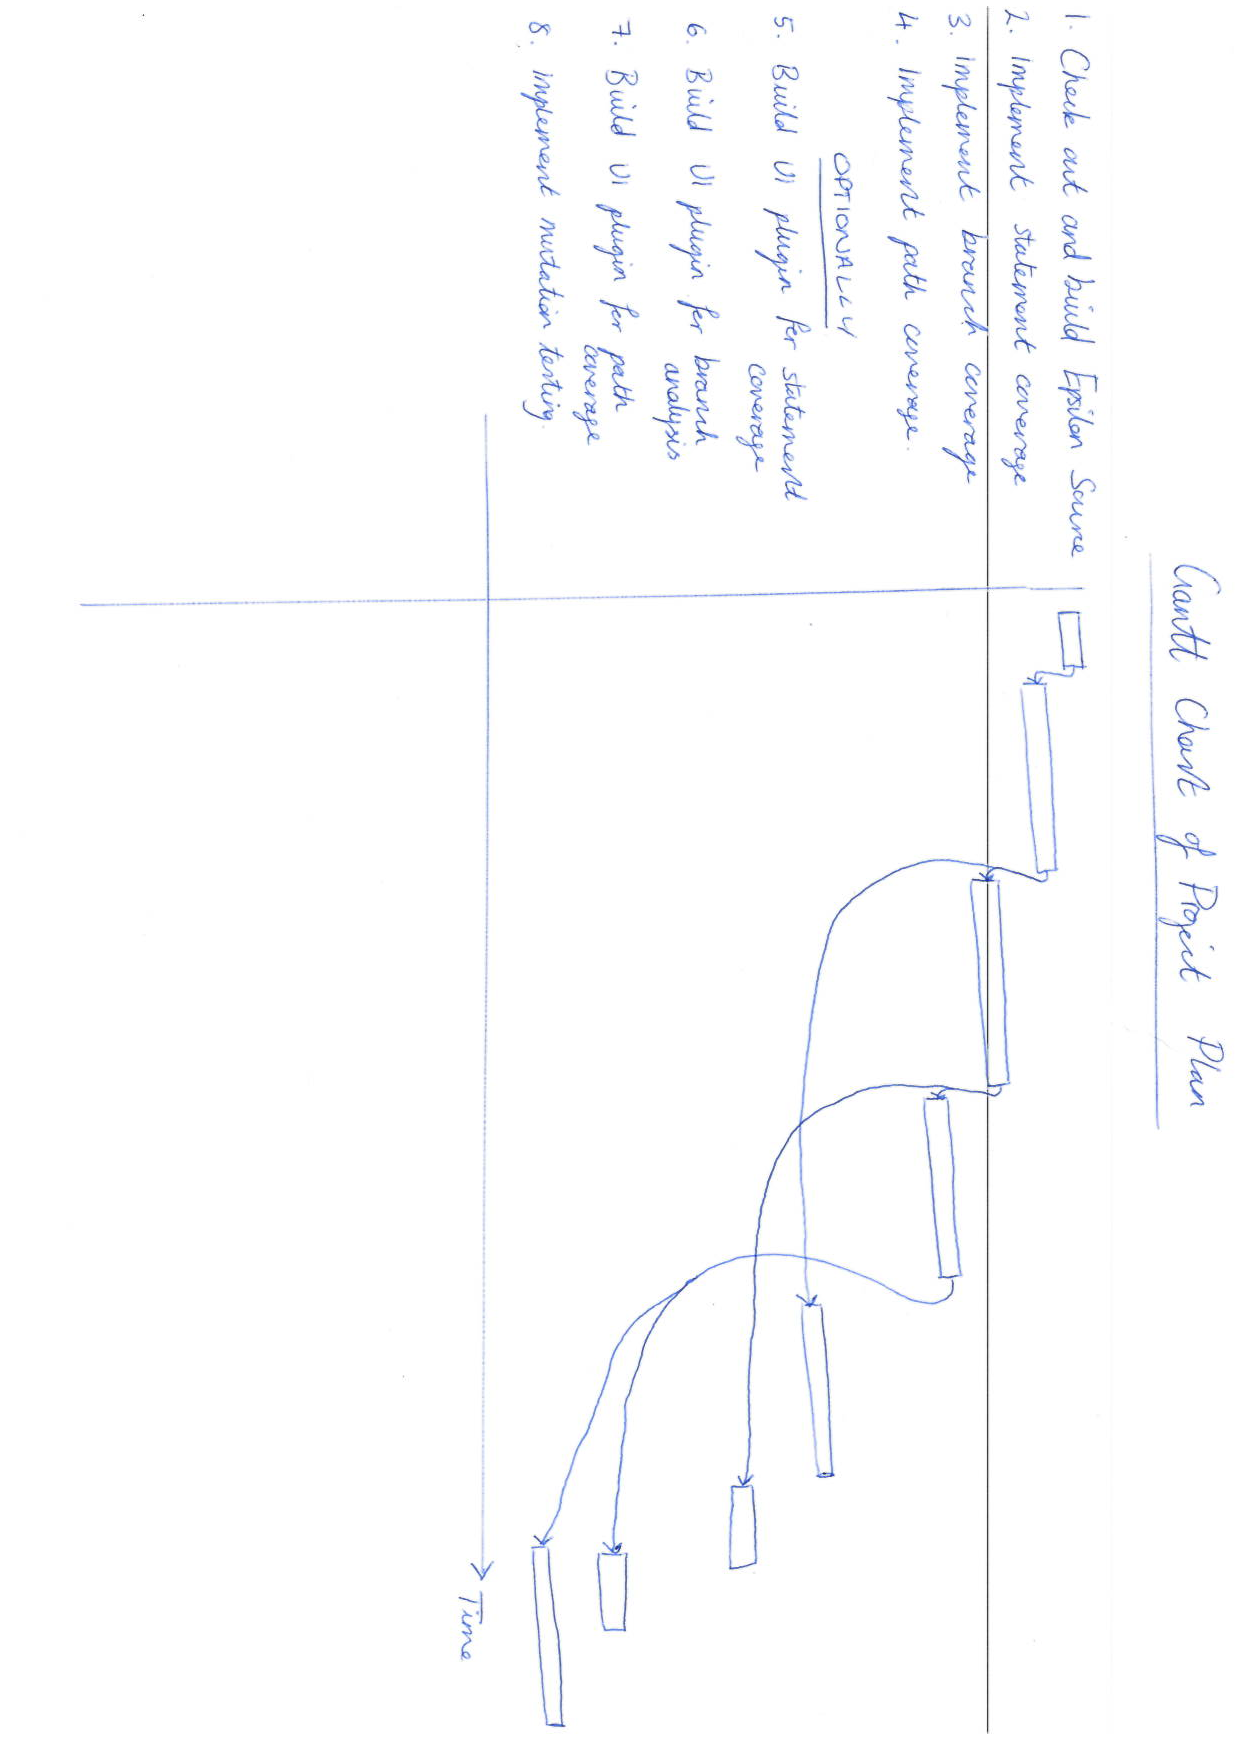
\includegraphics[scale=0.5]{figures/gantt.pdf}
\label{ganttChart}
\caption{A gantt chart of the project's expected progress}
\end{figure}